\section{Comparison}
\label{section:comparison}

<<<<<<< HEAD
\par Now a comparison between the theoretical analysis and the experimental analysis results of the gain is done.
 

\begin{figure}[H]
\centering
\begin{subfigure}{.5\textwidth}
  \centering
  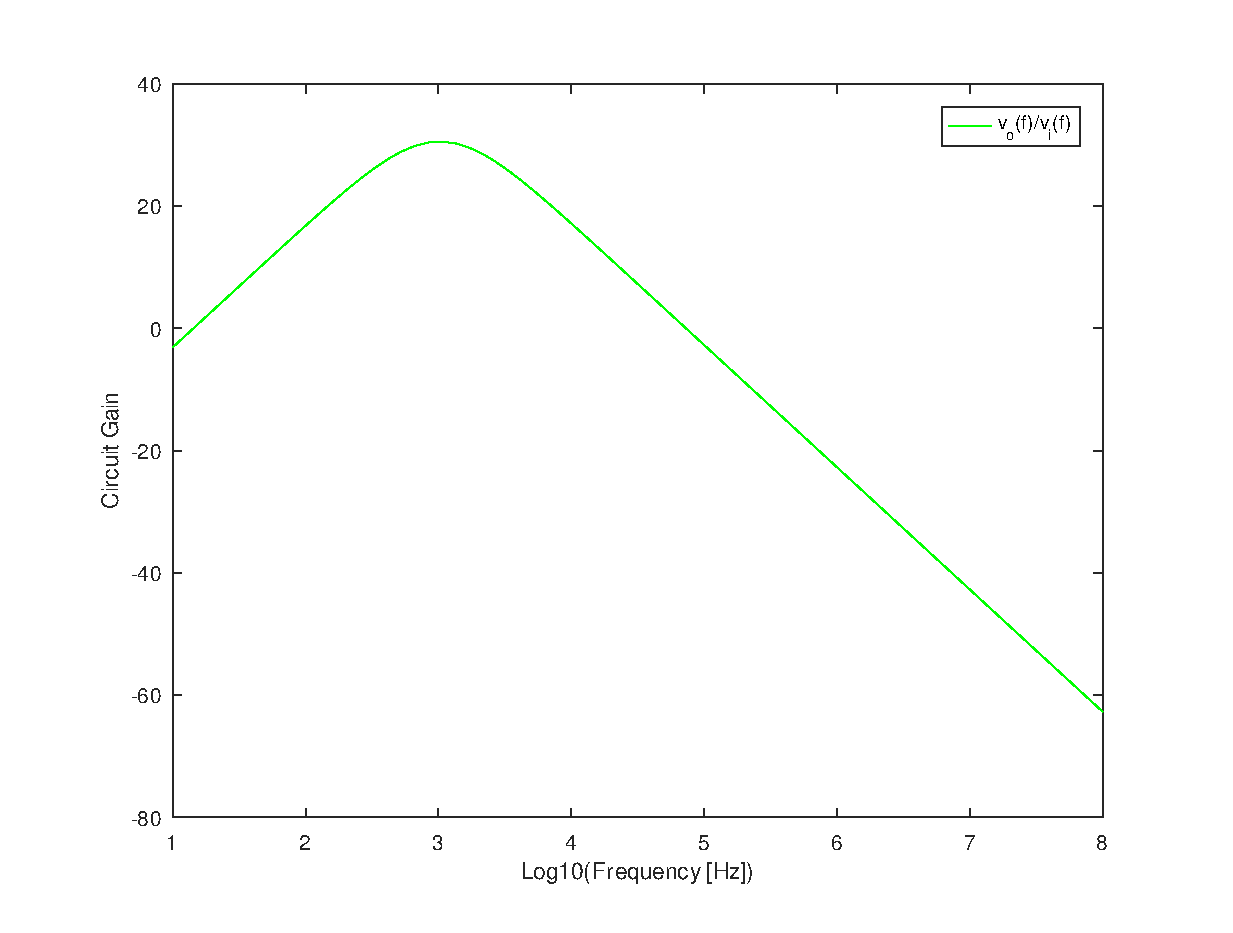
\includegraphics[width=1.1\linewidth]{teoria.eps}
  \caption{Output Voltage - Theoretical Model}
  \label{fig:sim4}
\end{subfigure}
\begin{subfigure}{.5\textwidth}
  \centering
  \includegraphics[width=1.1\linewidth]{vo2f.pdf}
  \caption{Output voltage - Ngspice model}
  \label{fig:sim5}
\end{subfigure}
\end{figure}

\par As we can see the graphics are pretty similar, which means that our theoretical model is a good approximation to the real running of an audio amplifier. Furthermore we can compare the values which we are studying and trying to improve: maximum gain and bandwidth and also a comparison between the operating point values is going to be made. The values are shown in the table below.

\begin{table}[H]
=======
\par Now a comparison between the theoretical analysis and the experimental analysis results is done and the results discussed conserning its accuracy and discrepancy. For the theoretical analysis as seen in the previous section an operating point analysis is mada in order to calculate the needed values.
 
 \par Conserning the passband frequency, we were able to obtain it using the function measure of ngspice. In the theoretical analysis it was calculated using the high and low pass band frequencies. Because of this the values are going to differ as we can see below.

 \begin{table}[h]
\parbox{.45\linewidth}{
  \centering
  \begin{tabular}{|l|r|}
    \hline    
    {\bf Calculus} & {\bf Value} \\ \hline
    V Gain&34.1403\\ \hline
Bandwidth&1.22339E+06\\ \hline
Lower Cut Off Freq& 15.8089\\ \hline
Higher Cut Off Freq& 1.22341E+06\\ \hline

  \end{tabular}
  \caption{Central frequency [Hz] and respective gain [dB]. (Ngspice)}} 
\parbox{.45\linewidth}{
 \centering
  \begin{tabular}{|l|r|}
    \hline    
    {\bf Name} & {\bf Value} \\ \hline
    \input{../mat/wo_freq_gain_TAB}
  \end{tabular}
  \caption{Central frequency [Hz] and respective gain [dB]. (Octave)}}
\end{table}

\par Also the input and output impedances were calculated in both analysis are now compared below in the tables shown.

\begin{table}[ht]
>>>>>>> d0b080297fc0b7e965087175cb535c02ef7a19c1
\parbox{.45\linewidth}{
  \centering
  \begin{tabular}{|l|r|}
    \hline    
<<<<<<< HEAD
    {\bf Calculus} & {\bf Value [V]} \\ \hline
    @gb[i] & -2.72859e-04\\ \hline
@id[current] & 1.035361e-03\\ \hline
@r1[i] & 2.604926e-04\\ \hline
@r2[i] & -2.72859e-04\\ \hline
@r3[i] & -1.23662e-05\\ \hline
@r4[i] & 1.248639e-03\\ \hline
@r5[i] & -1.30822e-03\\ \hline
@r6[i] & 9.881466e-04\\ \hline
@r7[i] & 9.881466e-04\\ \hline
v(1) & 1.216927e+01\\ \hline
v(2) & 7.480974e+00\\ \hline
v(3) & 8.035705e+00\\ \hline
v(4) & 8.297960e+00\\ \hline
v(5) & 3.074760e+00\\ \hline
v(6) & 1.005680e+00\\ \hline
v(7) & 8.073223e+00\\ \hline
v(8) & 1.005680e+00\\ \hline

  \end{tabular}
  \caption{Operating point - DC model (V) (Ngspice)}} 
=======
    {\bf Calculus} & {\bf Value [Ohm]} \\ \hline
    \input{../sim/Zin_tab}
  \end{tabular}
  \caption{Cirtcuit impedances. Variables are expressed in Ohm.(Ngspice)}} 
>>>>>>> d0b080297fc0b7e965087175cb535c02ef7a19c1
\parbox{.45\linewidth}{
 \centering
  \begin{tabular}{|l|r|}
    \hline    
<<<<<<< HEAD
    {\bf Name} & {\bf Value [V]} \\ \hline
    \input{../mat/ponto0_TAB}
  \end{tabular}
  \caption{Operating point - DC model (V) (Octave)}}
\end{table}

\par As we can see the values are close and the differences that exist may be explained because of the approximations done in the transistor models.
=======
    {\bf Name} & {\bf Value [Ohm]} \\ \hline
    \input{../mat/impedances_TAB}
  \end{tabular}
  \caption{Cirtcuit impedances. Variables are expressed in Ohm.(Octave)}}
\end{table}

\par As we can see the values are close and the differences that exist may be explained because of the approximations done in the amplifier model, as no IOS and VOS current and voltage were considered which means that only the ideal model of the transistor was considered. These sources are put in place as the resistance in the circuits' cables are bigger than zero which means that the current on the inputs of the amplifier isn't going to be null as we considered. Also the OP-Amp model used in the theoretical analysis consists of many simplifications which explain the differences shown above.
>>>>>>> d0b080297fc0b7e965087175cb535c02ef7a19c1
\newpage

